\documentclass[11pt]{article}

\usepackage[margin=0.8in]{geometry}
\usepackage{graphicx}
\usepackage{caption}
\usepackage{booktabs}
\usepackage{array}
\usepackage[hidelinks]{hyperref}
\usepackage{microtype}

\setlength{\emergencystretch}{2em}

\graphicspath{{figures/}}

\title{Expanded Segmentation Method Comparison and Proxy Benchmarking}
\author{}
\date{}

\begin{document}
\maketitle

\section*{Purpose and Scope}

This v2 package expands the segmentation-method comparison for the App80,
App65, and App81 organoid image datasets. It is saved separately from the first
comparison package so the earlier output remains unchanged. The expanded package
contains more source-matched examples, text-free figure grids, quantitative proxy
benchmarks, a heatmap-style summary figure, and source manifests.

The benchmarking is not a manual-ground-truth accuracy study. Instead, it is a
method-routing and quality-control comparison against the final AAPS-selected
mask for each source image. This framing is important because the final masks
were selected after method routing, visual QC, and human-in-the-loop correction;
they represent the selected analysis reference for metric extraction, not an
independent annotation standard.

\section*{Benchmark Definitions}

For each non-raw panel, the corresponding instance mask was compared with the
final AAPS-selected mask for the same source image. If mask grids differed, the
candidate mask was resized to the final mask grid using nearest-neighbour
interpolation before binary overlap was computed. The proxy metrics are:

\begin{itemize}
\item Dice to final: binary Dice overlap between the candidate mask and the final selected mask.
\item Area ratio to final: total candidate mask area divided by final mask area.
\item Instance-count delta: candidate instance count minus final instance count.
\item Small-fragment burden: fraction of mask area contained in very small connected components.
\item Edge-touch burden: fraction of mask area in components touching the image border.
\item Dominant-object fraction: fraction of mask area contained in the largest instance.
\end{itemize}

\begin{table}[p]
\centering
\small
\caption{Proxy benchmarking against the final AAPS-selected mask. Dice and area ratio are computed after nearest-neighbour resizing to the final mask grid when required. These values are QC/proxy metrics, not manual ground-truth accuracy.}
\begin{tabular}{llrrrrrr}
\toprule
Dataset & Method & n & Dice & Area ratio & $\Delta$ count & Small frag. & Edge touch \\
\midrule
App80 & Prompted watershed & 7 & 0.11 & 0.03 & -9 & 0.0\% & 0.0\% \\
App80 & CPSAM & 7 & 0.07 & 0.03 & -7 & 0.0\% & 0.0\% \\
App80 & Final multiscale & 7 & 1.00 & 1.00 & +0 & 0.0\% & 0.0\% \\
App65 & Old multiscale & 6 & 0.75 & 1.26 & -6 & 0.0\% & 34.4\% \\
App65 & Threshold-hinted Cellpose & 6 & 0.75 & 1.49 & -0 & 0.0\% & 94.8\% \\
App65 & Final direct brightfield & 6 & 1.00 & 1.00 & +0 & 0.0\% & 9.9\% \\
App81 & Threshold-hinted Cellpose & 5 & 0.36 & 0.67 & -2 & 0.0\% & 0.0\% \\
App81 & Resized multiscale Cellpose & 5 & 0.26 & 0.92 & +0 & 0.0\% & 0.0\% \\
App81 & Image-generation mask & 5 & 0.48 & 0.89 & +1 & 2.1\% & 0.0\% \\
App81 & Final stitched hybrid & 5 & 1.00 & 1.00 & +0 & 0.0\% & 0.0\% \\
\bottomrule
\end{tabular}
\end{table}


\section*{Visual QC Assessment from Image Review}

The expanded figures were reviewed directly using the Codex image viewer. The
main observations are consistent across the visual grids and the proxy metrics.

\textbf{App80 Y-27632.} The early prompted-watershed and CPSAM/SAM-style columns
often capture only small local regions or partial edges. In later 10~uM images,
they miss large organoid-scale structures almost completely. The final
multiscale large-recovery branch recovers the biologically relevant large
objects, including broad fused structures. This is the correct direction for
growth and recovery metrics, but it also means the final branch should be
described as a deliberate large-object recovery strategy rather than a universal
manual-like contour.

\textbf{App65 alginate.} The old multiscale branch frequently expands into
broad irregular masses around dense brightfield structures. The threshold-hinted
Cellpose branch gives cleaner separated candidates in some images, but the
reviewed grid shows strong edge-touching and broad peripheral masks in several
fields. The final direct-brightfield branch is more conservative and
instance-like, which is better aligned with perimeter, wall-darkness, and
peripheral/central measurements.

\textbf{App81 density.} This dataset shows why AAPS method routing is necessary.
Threshold-hinted and resized multiscale Cellpose can both mistake large pale
droplet boundaries for organoids, especially in low-density panels, or miss true
cystic organoids when the size prior is wrong. Image-generation-assisted masks
are semantically useful for recognizing cystic structures, but reviewed examples
also show stylized masks, merged large objects, and non-final mask geometry. The
final stitched hybrid output is the most controlled representation because it
uses panel-level method selection and human-in-the-loop replacement only where a
candidate method improves the selected mask.

\begin{figure}[p]
\centering
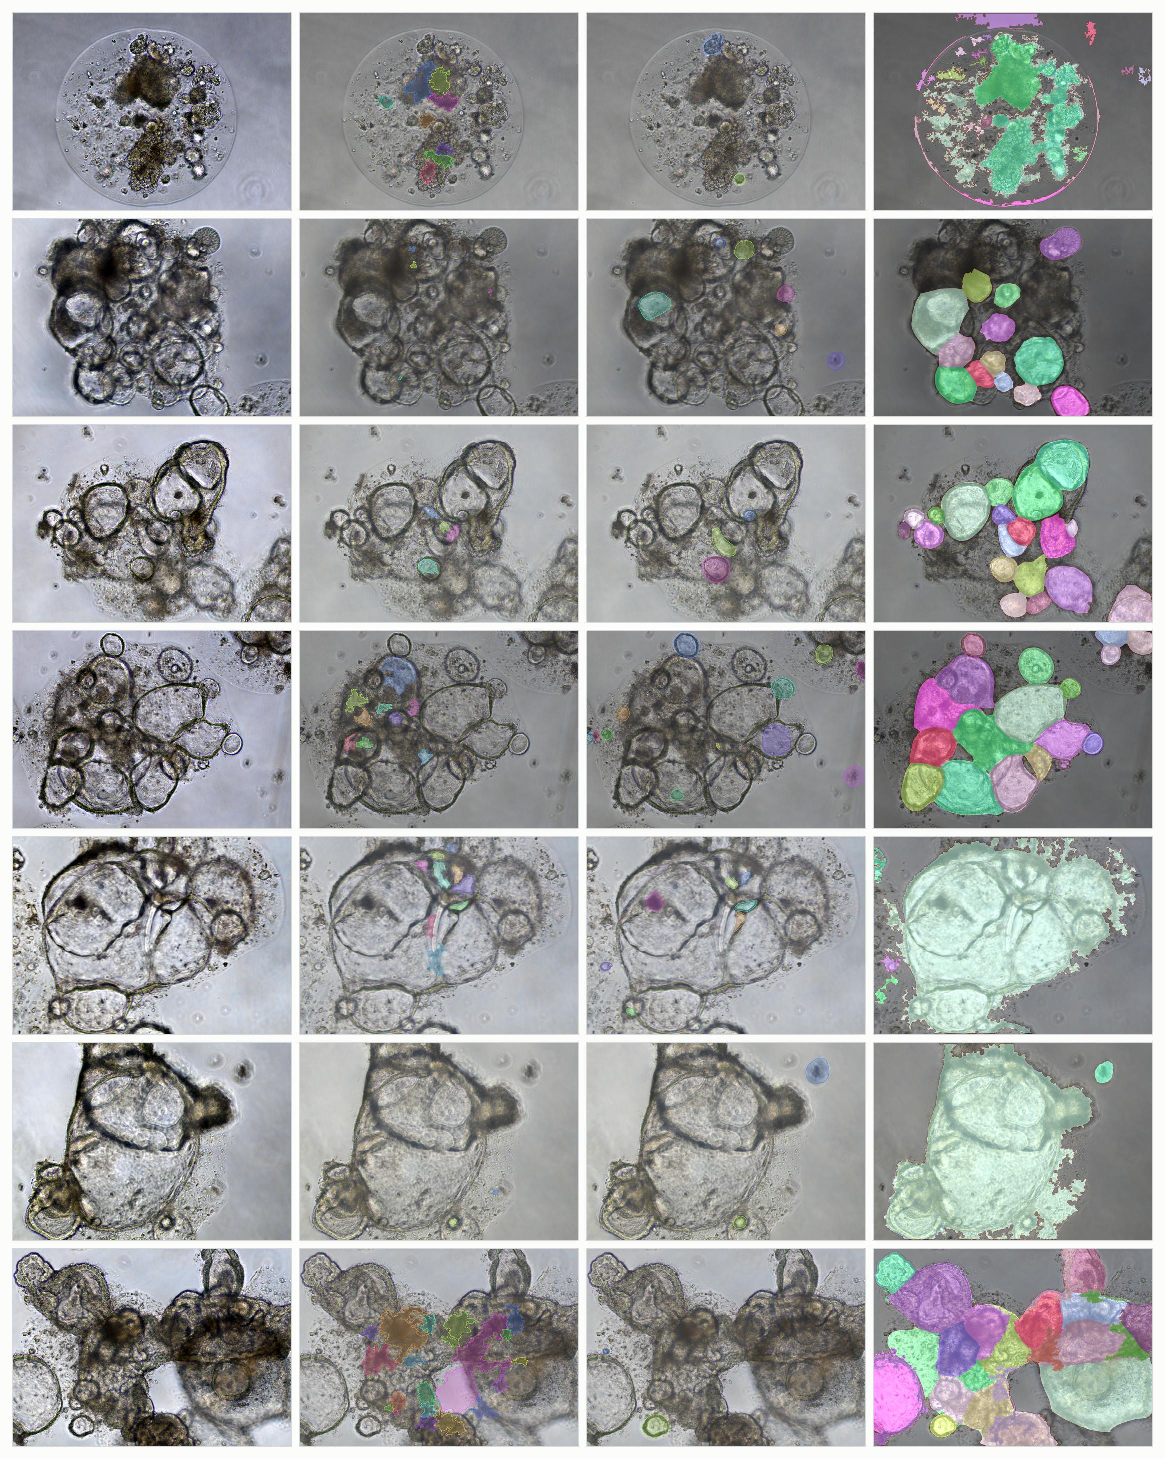
\includegraphics[width=\textwidth,height=0.78\textheight,keepaspectratio]{app80_method_comparison_v2_no_text.pdf}
\caption{\textbf{Expanded App80 Y-27632 segmentation comparison.}
Rows show seven source-matched 10~uM Y-27632 fields from 5, 7, 8, 9, 10, 11,
and 12 December 2025. Columns show, from left to right: raw brightfield image,
early prompted-watershed overlay, early CPSAM/SAM-style proposal overlay, and
the final AAPS multiscale large-object recovery overlay. The no-text grid shows
that early methods tend to under-cover the large organoid structures that emerge
during recovery, while the final branch intentionally recovers larger connected
organoid-scale objects for downstream growth and fusion-related metrics.}
\end{figure}

\begin{figure}[p]
\centering
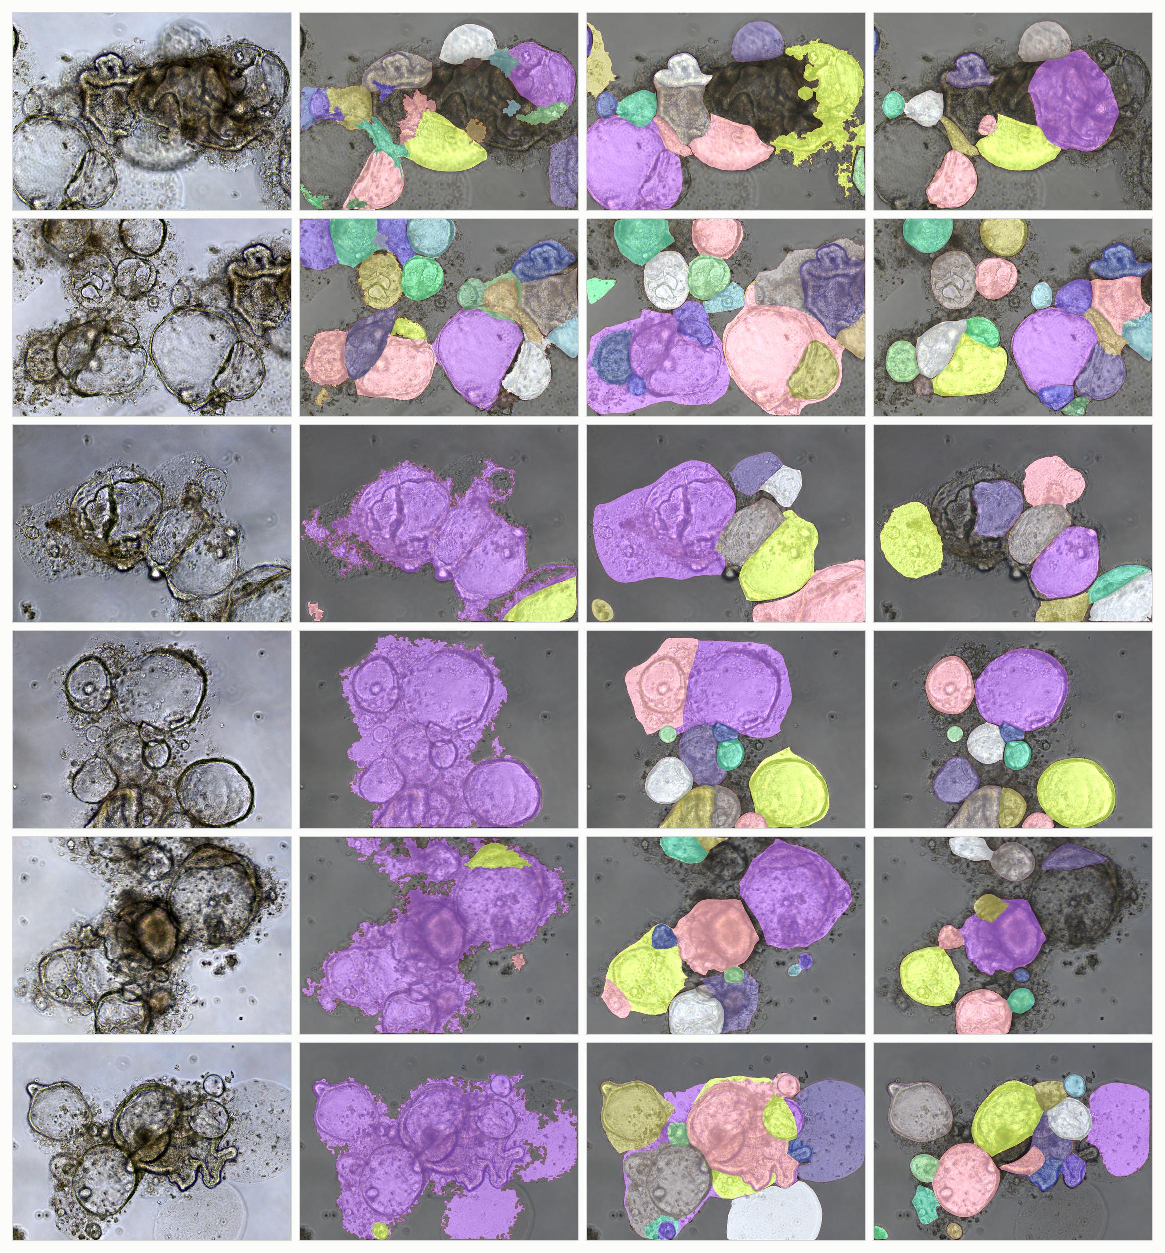
\includegraphics[width=\textwidth,height=0.78\textheight,keepaspectratio]{app65_method_comparison_v2_no_text.pdf}
\caption{\textbf{Expanded App65 alginate segmentation comparison.}
Rows show six 0.02\% alginate fields from 29 November 2025: 10x00, 10x01,
10x14, 10x15, 10x16, and 10x17. Columns show, from left to right: raw
brightfield image, old multiscale Cellpose recovery overlay, threshold-hinted
Cellpose overlay, and final AAPS direct-brightfield overlay. The comparison
shows that the final branch is more conservative and instance-like than the old
large-recovery branch, while avoiding much of the edge-touching burden seen in
the threshold-hinted results.}
\end{figure}

\begin{figure}[p]
\centering
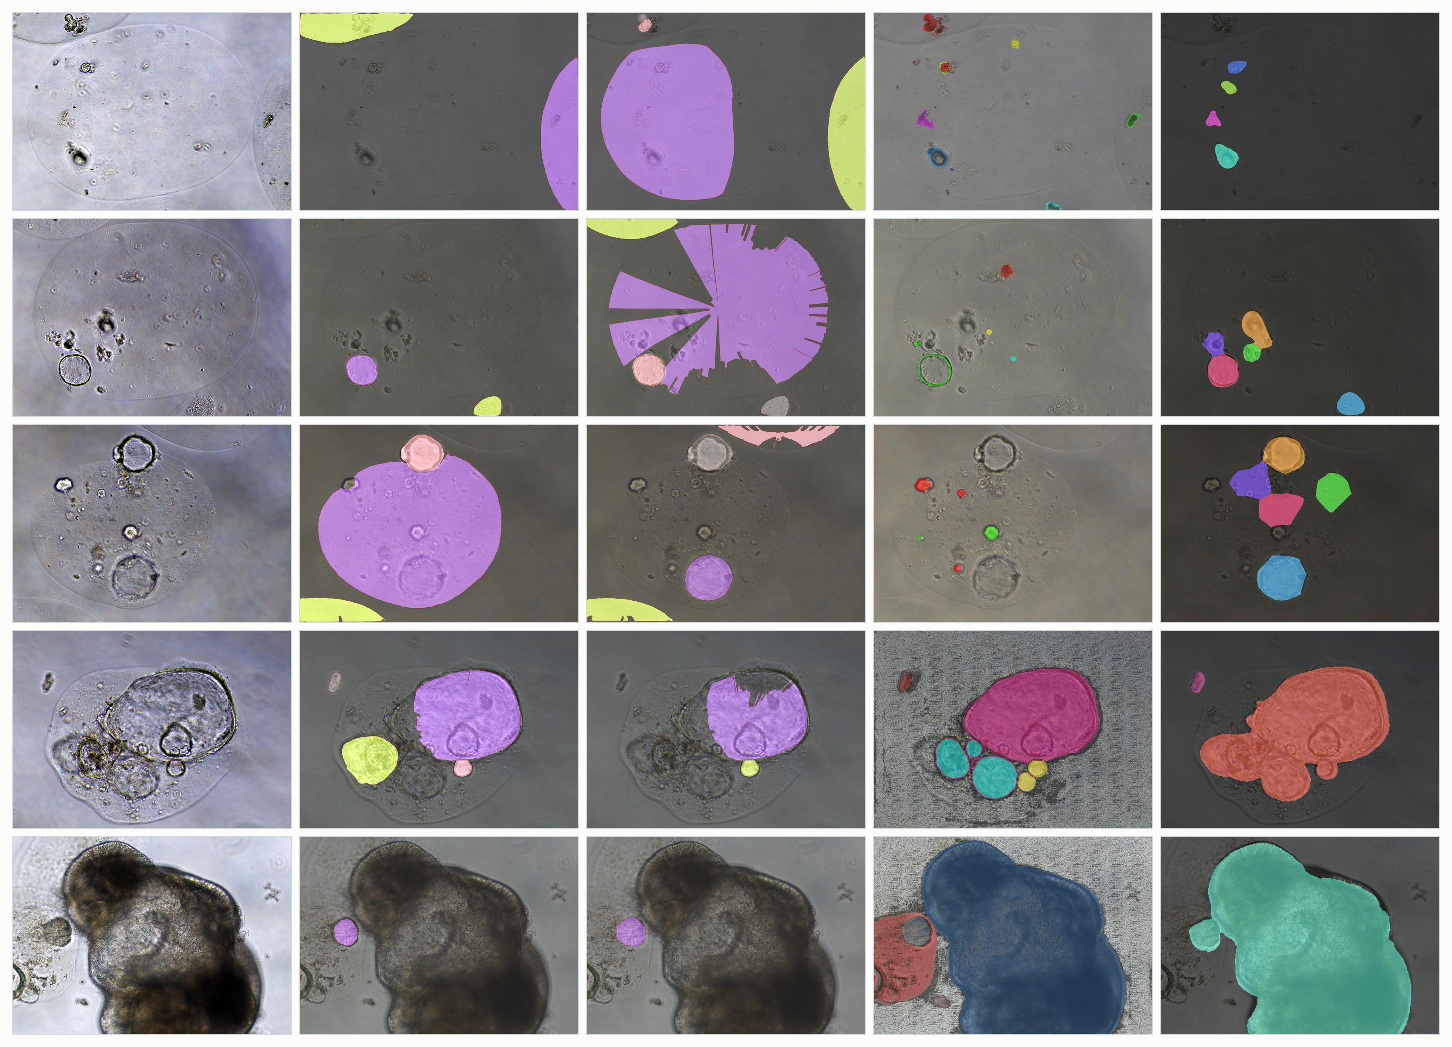
\includegraphics[width=\textwidth,height=0.78\textheight,keepaspectratio]{app81_method_comparison_v2_no_text.pdf}
\caption{\textbf{Expanded App81 density method-routing comparison.}
Rows show five source-matched App81 examples: low-density fields from 14, 15,
and 16 October 2025, followed by middle-density fields from 18 and 29 October
2025. Columns show, from left to right: raw brightfield image, threshold-hinted
Cellpose, resized multiscale Cellpose, image-generation-assisted mask, and final
stitched AAPS-selected hybrid overlay. The grid shows that no single method is
stable across density, droplet-boundary ambiguity, cystic size range, and large
dark organoids. Image generation adds semantic recognition, but the final
analysis mask still requires AAPS-style QC and method selection.}
\end{figure}

\begin{figure}[p]
\centering
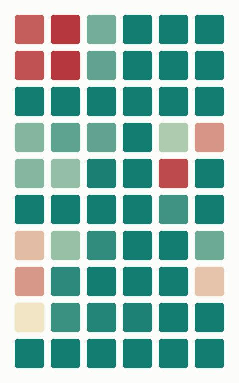
\includegraphics[width=0.44\textwidth]{proxy_benchmark_heatmap_v2_no_text.pdf}
\caption{\textbf{Text-free proxy benchmark heatmap.}
Rows follow the order of the benchmark table: App80 prompted watershed, App80
CPSAM, App80 final multiscale, App65 old multiscale, App65 threshold-hinted
Cellpose, App65 final direct-brightfield, App81 threshold-hinted Cellpose,
App81 resized multiscale Cellpose, App81 image-generation mask, and App81 final
stitched hybrid. Columns show, from left to right: Dice-to-final score,
area-ratio agreement, instance-count agreement, low-fragment score, low-edge
touch score, and low-dominant-merge score. Teal indicates stronger agreement or
lower QC burden; red indicates weaker agreement or higher QC burden.}
\end{figure}

\section*{Interpretation for the Manuscript}

The expanded comparison supports the AAPS claim that robust organoid
quantification requires method routing rather than one fixed segmentation
algorithm. App80 required large-object recovery because the biological endpoint
is growth and recovery under Y-27632. App65 required a more conservative
direct-brightfield branch because perimeter and wall-darkness metrics are
sensitive to edge-touching and broad masks. App81 required a stitched hybrid
strategy because cystic organoid identity, droplet-boundary exclusion, and
instance separation varied substantially across density panels.

The quantitative proxy results provide a compact way to report these routing
decisions. For App80, early watershed and CPSAM masks show very low overlap and
area relative to the final selected masks, reflecting severe under-coverage of
large structures. For App65, old and threshold-hinted branches have moderate
Dice-to-final values but substantially higher area ratios or edge-touch burdens,
matching the visual over-expansion seen in the grids. For App81,
image-generation-assisted masks align better with the final selected masks than
the tested Cellpose variants on these examples, but the visual review shows why
image generation was not used unguarded: it still requires cleanup, splitting,
and panel-level selection.

\end{document}
